% Options possibles
% init - pour le dossier d'initialisation
% francais ou english
% RandD - réservé aux PFE ayant le label R&D.
% Confidential - réservé aux PFE confidentiels
\documentclass[francais]{rapportPFE}  % pour une version française
%\documentclass[english]{rapportPFE}  % pour une version avec du texte en anglais

% L'option confidentiel a pour conséquence d'ajouter le filigrane "Confidentiel" sur la première et la dernière page
%  En fait, ce filigrane apparait sur toutes les pages numérotées 1 par Latex… 
% Pour le rajouter sur TOUTES les pages, décommenter la commande suivante
%\newwatermark[allpages,textalign=center,fontfamily=pbk,angle=55,scale=2.75,xpos=-1cm,ypos=1cm,color=lightgray]{Confidentiel}



\usepackage{listings}
\usepackage{fancyhdr}
% %%%%%%%%%%%%%%%%%%%%%%%%%%%%%%%%%%%%%%%%%%%
% titres du rapport
% %%%%%%%%%%%%%%%%%%%%%%%%%%%%%%%%%%%%%%%%%%%
% Version francaise
\titre{Développement d’interface graphique technologie web - faisabilité et évaluation}
% version anglaise
\title{Development of web-based graphical user interface - feasibility and evaluation}


% %%%%%%%%%%%%%%%%%%%%%%%%%%%%%%%%%%%%%%%%%%%
% Auteur du rapport
% %%%%%%%%%%%%%%%%%%%%%%%%%%%%%%%%%%%%%%%%%%%
\firstname{Colin}
%\middlename{Autre-Prénom}
\lastname{Thomas}



% %%%%%%%%%%%%%%%%%%%%%%%%%%%%%%%%%%%%%%%%%%%
% Informations sur le PFE
% %%%%%%%%%%%%%%%%%%%%%%%%%%%%%%%%%%%%%%%%%%%
% Information administratives
\dateDebutPFE{5 février 2024}
\dateFinPFE{26 juillet 2024}
\nomStructureAcceuil{Arturia}
\villeStructureAccuel{Grenoble}
\logoStructureAccueil{width=5.0cm}{graphics/LogoStructureAccueil} % si vous ne souhaitez pas mettre de logo pour la structure d'accueil, commentez cette ligne.
% paramètres de la commande logoStructureAccueil
% #1 = paramètre d'affichage du logo
% #2 = nom du fichier logo
% Pour plus de précision, cela correspond à la commande latex \includegrahics[#1]{#2}

% Encadrants.
% Penser à accorder la fonction avec le genre
\begin{encadrants}
% Fonction {Fonction}{ Prénom \Nom{Nom}}{Titre}{Structure}
  \referent{Référent}{Yann \Nom{Gripay}}{Maître de Conférences}{INSA Lyon}%
  \tuteur{Tuteur}{Timothée \Nom{Béhéty}}{Référent Technique Logiciels Compagnon}{Arturia (Grenoble)}
\end{encadrants}

% Date de la soutenance
\date{26 juin 2020}

% Réglage des entêtes et pieds de page
\fancyhf{}
\renewcommand{\headrulewidth}{0.2pt}
\renewcommand{\footrulewidth}{0.2pt}
\fancyhead[L]{\footnotesize{Un exemple d'en-têtes 
     et pieds de page}}
\fancyfoot[R]{\thepage}
\fancyfoot[C]{\footnotesize{---}}
\fancyfoot[L]{\footnotesize{\textit{Les 
     rédacteurs de la FAQ}}}


% %%%%%%%%%%%%%%%%%%%%%%%%%%%%%%%%%%%%%%%%%%%
% Rapport lui même
% %%%%%%%%%%%%%%%%%%%%%%%%%%%%%%%%%%%%%%%%%%%
\begin{document}
\maketitle


% ==========================================
% les résumés et les mots clés du rapport
% ==========================================

\begin{ResumeMotsCles}

% Version anglaise
% abstract no more than 12 lines.
\begin{resumeEn}
During my final internship, I had the opportunity to participate in the design and development of web interfaces for Arturia's next generation Companion Softwares. These softwares include the Arturia Software Center, Arturia's software store, and the Midi Control Center, Arturia's hardware configuration software. With the aim of updating aging software and experimenting with new graphic development technologies, my team decided to prototype a modular application bringing them together, utilizing web interfaces for the front-end.\\
My role involved developing web interfaces for the Arturia Software Center, integrating a C++ back-end developed by another team member. I also redesigned the Midi Control Center and prototyped the use of the Web MIDI API to communicate with Arturia devices on the web, as well as experimenting with the Web USB API to update device firmware.\\
Throughout my internship, I followed and participated in the conception of the modular application during weekly architecture meetings. \\
Working on such an innovative project at Arturia allowed me to explore innovative domains and deepen my teamwork and communication skills, which I had developed during my previous internships. 
\end{resumeEn}
% keywords
\keywords{Web~; Vue Nuxt~; Cross-Plateform~; Web APIs~; Modular App.}



% Version francaise
% Résumé pas plus de 12 lignes
\begin{resumeFr}
Durant mon stage de fin d'études, j'ai pu participer à la conception et au développement d'interfaces Web pour la nouvelle génération des Logiciels Compagnon d'Arturia. Ces logiciels sont l'Arturia Software Center, le magasin de logiciels d'Arturia, et le Midi Control Center, le logiciel de configuration de matériel Arturia. Dans l'optique de mettre à jour des logiciels vieillissant, et d'expérimenter de nouvelles technologies de développement graphique, mon équipe a décidé de prototyper une application modulaire les rassemblant, et d'utiliser des interfaces Web pour la partie front-end. \\% //TODO : modifier texte précédent
Mon rôle a été de développer des interfaces Web pour l'Arturia Software Center, en y intégrant un back-end C++ développé par un autre membre de l'équipe. J'ai également réalisé un nouveau design pour le Midi Control Center, et ai pu prototyper l'utilisation de l'API Web MIDI pour communiquer avec les appareils Arturia.  \\
J'ai pu par ailleurs, au long de mon stage, suivre et participer à la conception de l'application modulaire lors de réunions d'architecture hebdomadaires.\\
Travailler sur un projet aussi innovant à Arturia m'a permis d'expérimenter des domaines novateurs, mais aussi d'approfondir mes compétences de travail en équipe et de communication que j'ai pu développer lors de mes précédents stages. 
\end{resumeFr}

% Mots clés
\motscles{Web~; Vue Nuxt~; Cross-Plateforme~; Web APIs~; Application Modulaire.}
\end{ResumeMotsCles}


% ==========================================
% Remerciements éventuels
% ==========================================
% \begin{remerciements}
%   Merci à tous. Commenter cet environnement s'il n'est pas nécessaire.
% \end{remerciements}





% %%%%%%%%%%%%%%%%%%%%%%%%%%%%%%%%%%%%%%%%%%
% rapport proprement dit 
% %%%%%%%%%%%%%%%%%%%%%%%%%%%%%%%%%%%%%%%%%%

% ==========================================
% Sommaire (généré automatiquement)
% ==========================================
\setcounter{tocdepth}{3}
\tableofcontents
\cleardoublepage

% ==========================================
% Introduction
% ==========================================
%Contexte, 
%définition du problème, 
%aperçu des contributions, 
%plan du rapport



     
     
     
\section{Introduction.}

\subsection{Mise en contexte.}
\subsection{Définition du problème.}
\subsection{Aperçu des contributions.}
\subsection{Problématique et plan.}



\section{Contexte.}

\subsection{Contexte du stage.}
\subsection{Arturia.}

Arturia est un fabricant d'instruments de musique numériques et électroniques. La société est basée à Grenoble et développe des reproductions logicielles d'anciens synthétiseurs (analogiques et numériques), des claviers MIDI, des contrôleurs, des synthétiseurs analogiques et des interfaces audio. 

Il s'agit d'une entreprise employant 180 personnes, qui a été fondée en 1999. A sa création, ses deux fondateurs Frédéric Brun (actuel PDG d'Arturia) et Gilles Pommereuil ont commencé par créer des reproductions de synthétiseurs analogiques réputés au format virtuel, en commençant par développer l'Analog V, inspiré par les synthétiseurs Moog et en collaboration avec leur créateur. De nombreuses autres reproductions ont suivi, et sont devenues par la suite la V Collection, qui est la collection d'instruments virtuels d'Arturia, et la FX Collection, qui est son équivalent pour les effets audio.

Arturia a depuis élargi son catalogue à des instruments virtuels qui lui sont propres, plusieurs synthétiseurs analogiques renommés, différents contrôleurs MIDI ainsi que des cartes sons. 

L’équipe Compagnon dans laquelle je réalise mon stage s’occupe des logiciels accompagnants les produits Arturia, comme le gestionnaire de licences, le logiciel de configuration de matériel, ou encore des logiciels spécifique à chaque produits, comme par exemple l'application mobile qui accompagne le clavier AstroLab. 

\subsection{Présentation du sujet de stage.}


\subsubsection{Mission.}

L'Arturia Software Center (ASC) et le Midi Control Center (MCC) sont deux logiciels vieillissants, qu'Arturia souhaite mettre à jour. Pour faire cela, l'entreprise souhaite mettre à l'épreuve de nouvelles technologies de développement graphique.

En effet, ces logiciels ont été développés respectivement en 2014 pour l'Arturia Software Center, et en 2013 pour le Midi Control Center. A ce moment, l'équipe Compagnon que j'intègre pour ce stage n'existait pas encore, et ces logiciels ont donc étés développés par l'équipe Software, qui se spécialise dans le développement d'instruments virtuels. Ils ont opté pour l'utilisation de technologies de développement d'instruments virtuels, notamment le framework C++ JUCE, pour la création de ces outils. Cependant, une mise à jour de l'ASC et du MCC en utilisant des technologies différentes permettrait de se détacher des outils spécifiquement conçus pour les logiciels audio, potentiellement inadaptés à ces applications.

Ainsi, l'équipe Compagnon a décidé de prototyper une application modulaire qui rassemblerait l'Arturia Software Center et le Midi Control Center. Cette application serait capable de lancer des librairies C++ en tant que back-end, de servir en HTTP des pages Web statiques en tant que front-end, et d'afficher un host permettant de naviguer sur ces pages Web. De cette manière, l'Arturia Software Center et le Midi Control Center constitueraient = deux modules de cette application, chacun dotés d'un back-end sous forme de librairie C++, et d'un front end sous forme de page web statique, communiquant avec leur back-end par requêtes HTTP.\\

\subsubsection{Intérêt.}

Utiliser des interfaces web pour ces logiciels se révèle ainsi positif sur plusieurs points : 
\begin{itemize}
	\item Les technologies web sont plus efficaces pour créer rapidement des interfaces. En effet, les bibliothèques et outils pré-développés et libres d'accès sont nombreux, en constante évolution, et facile d'utilisation : on peut prendre pour exemple la fonctionnalité multilangue, qui est une fonctionnalité qui prend de l'importance pour Arturia, et qui demande beaucoup de ressources, pour un développement plus facile, classique et très documenté en technologies Web. De même, les framework Web offrent souvent une courbe d'apprentissage plus faible que le C++ ou autre langage qui n'est pas haut-niveau.
	\item Ceci permet, pour développer ces interfaces, de pouvoir rechercher des profils de développeurs front-end Web, ce qui est plus facile que de devoir rechercher des développeurs C++, puis de les former sur le framework JUCE, pour ensuite travailler sur des interfaces. En séparant le développement front-end du reste de l'application, ceci permet de rechercher des développeurs spécialisés dans leur domaines, et ainsi une meilleure évolutivité de l'équipe.
	\item Ensuite, cela permet de séparer le front-end du back-end. En effet, avoir une interface HTTP entre un back-end et un front-end permet de bien séparer ces deux parties. Ceci amène de la modularité et de la scalabilité, car chaque partie peut être modifiée sans affecter l'autre. On peut imaginer également une plus grande flexibilité technologique, car l'application Web pourrait être développée dans n'importe quel framework, sans impliquer de changement pour les librairies C++. Enfin, en isolant les accès directs au back-end, on peut ainsi mettre en place de meilleurs mesures de sécurité pour protéger les logiciels et les licences utilisateurs.
\end{itemize}

L'Arturia Software Center étant l'outil qui permet de gérer l'installation des logiciels, un back-end est forcément nécessaire pour soutenir le front-end. En effet, par design et pour des raisons de sécurités, les technologies Web n'ont pas accès au système de fichiers de l'utilisateur.

En revanche, la question se posera pour le Midi Control Center, dont la principale fonctionnalité est de communiquer par protocole Midi avec le contrôleur. Nous étudierons pendant ce stage la faisabilité d'un Midi Control Center entièrement réalisé en technologies Web.

\section{Etude bibliographique et analyse de l'existant.}
\subsection{L'Arturia Software Center existant.}

L’Arturia Software Center
\footnote{\url{https://www.arturia.com/support/asc-arturiasoftwarecenter}}
 (ASC) est le logiciel de gestion de licences et de
téléchargement de software d’Arturia : il est nécessaire pour tout utilisateur
souhaitant utiliser un logiciel Arturia. L'utilisateur peut naviguer parmi les logiciels disponibles sur l'Arturia Software Center sur la page "Explore Products", activer la licence du logiciel sur la page "My Products", le télécharger, le mettre à jour, gérer l'emplacement de ses fichiers dans les paramètres, ainsi que de rentrer le code d'un produit Arturia physique afin de bénéficier des logiciels qui l'accompagnent.

L’Arturia Software Center est composé de deux parties : 

Tout d'abord, une partie principale, qui est ce logiciel qui permet de gérer ses licences et ses téléchargements de logiciels Arturia, et fournit une interface graphique.

Ensuite, un logiciel nommé ASC Agent, qui fonctionne en arrière plan, et vérifie les licences utilisateur à chaque démarrage de produit Arturia, afin d'éviter toute fraude et téléchargement illégal.

\begin{figure}[!t]
	\centering
	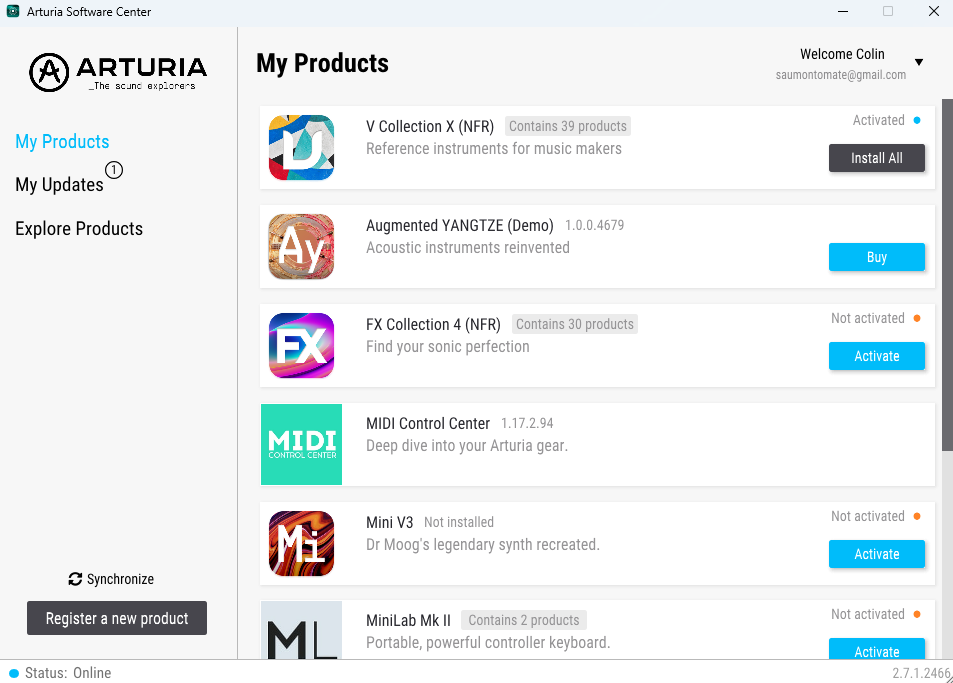
\includegraphics[width=0.6\textwidth]{graphics/asc_existant.png}
	\begin{tiny}
	\end{tiny}
	\caption{Arturia Software Center (ASC) existant}
	\label{fig:Expe}
\end{figure}

\subsection{Le Midi Control Center existant.}

Le Midi Control Center
\footnote{\url{https://support.arturia.com/hc/fr-fr/sections/4405740766098-MIDI-Control-Center}}
 (MCC) est le logiciel de configuration de matériel Arturia : il
permet de gérer les configurations et les paramètres des synthétiseurs et contrôleurs MIDI, ainsi que de faire les mises à jour firmware pour les synthétiseurs analogiques, cartes sons et claviers midis physiques d’Arturia. Il communique en norme MIDI avec les produits Arturia pour leur configuration.

Il est composé d'une page "Device Settings" permettant de modifier les paramètres généraux du contrôleur actuellement connecté (par exemple, son temps de mise en veille ou ses courbes de vélocité), une page "Controller Map" permettant de modifier les paramètres de chaque contrôle du contrôleur, (par exemple, modifier la note attribuée à une touche en particulier), et une page permettant d'importer ou d'exporter des templates de paramètres. Il est également possible d'effectuer une détection automatique de mises à jour disponibles pour le firmware du contrôleur.

\begin{figure}[!t]
	\centering
	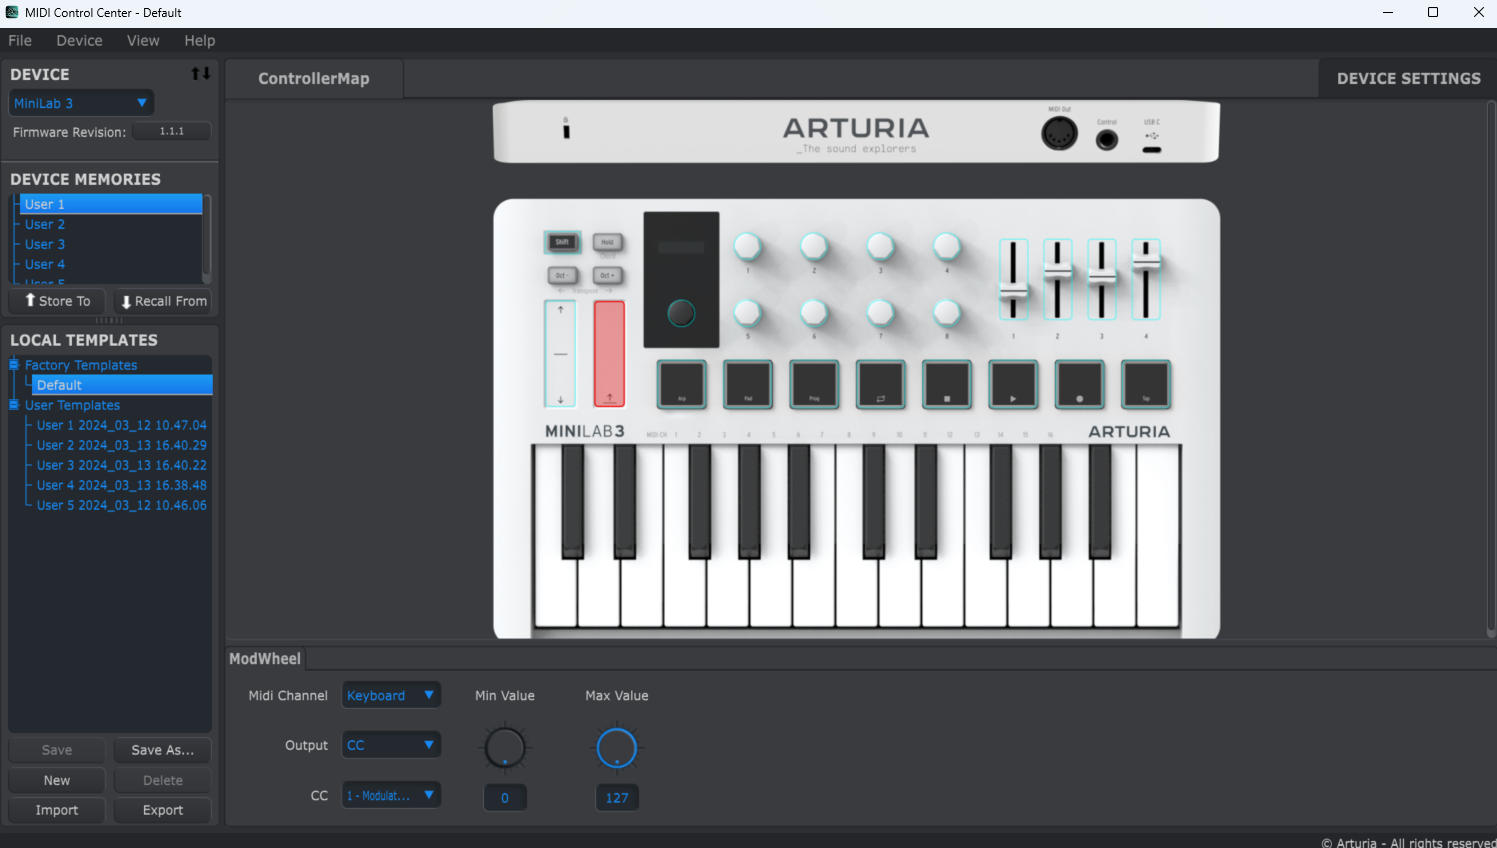
\includegraphics[width=0.6\textwidth]{graphics/mcc_existant.png}
	\begin{tiny}
	\end{tiny}
	\caption{Midi Control Center (MCC) existant}
	\label{fig:Expe}
\end{figure}


\subsection{L'API Web MIDI.}

L'API Web MIDI
\footnote{\url{https://developer.mozilla.org/en-US/docs/Web/API/Web_MIDI_API}}
fournit une manière pour les applications web d'interagir avec les périphériques MIDI connectés à l'ordinateur. Elle permet d'envoyer et de recevoir des messages MIDI, par exemple recevoir des messages de Note On / Note Off, mais aussi envoyer des messages Sysex permettant de modifier les paramètres du périphérique.

Cette API n'est pour l'instant disponible que sur les navigateurs Safari et Chromium. Ceci ne nous posera pas problème, car le fait que nous implémentons nous même le navigateur nous permet de le choisir. En l'occurence, celui que nous utilisons est celui de Juce, et il est basé sur Chromium pour Windows, et sur Safari pour Mac.


\subsection{Définitions nécessaires.}

Nous allons ici définir quelques termes propres au matériel de production musicale.
\paragraph{Synthétiseur analogique} \footnote{\url{https://fr.wikipedia.org/wiki/Synthétiseur_analogique}} 
:
 Un synthétiseur analogique est un synthétiseur qui utilise des circuits analogiques et des signaux électriques analogiques pour générer des sons par des techniques électroniques. Contrairement à un synthétiseur numérique, qui stocke et communique l'information en binaire, l'information sonore est transmise dans l'analogique en tant que variation de tension.
\paragraph{MIDI} \footnote{\url{https://fr.wikipedia.org/wiki/Musical_Instrument_Digital_Interface}} 
: Le Musical Instrument Digital Interface ou MIDI est un protocole de communication et un format de fichier dédiés à la musique, et utilisés pour la communication entre instruments électroniques, contrôleurs, séquenceurs, et logiciels de musique. Il s'agit du protocole standard du matériel électronique de musique. Il permet par exemple à un Contrôleur MIDI d'envoyer le signal qu'une certaine note a été pressée avec une certaine vélocité, permettant à un logiciel sur ordinateur de produire un son en conséquence. Dans le sens inverse, ce protocole permet à l'utilisateur de paramétrer son contrôleur MIDI en envoyant des signaux SYSEX, comportant les informations nécessaire sur le paramètre à modifier et la valeur à lui attribuer.
\paragraph{Contrôleur MIDI} \footnote{\url{https://troidecis.fr/musique/instrument-midi-definition}} 
:  Un contrôleur MIDI est un appareil utilisé pour envoyer des signaux MIDI à l'ordinateur où à un autre appareil (par exemple, un synthétiseur analogique). Il peut se présenter sous la forme d'un clavier de piano, de faders, de potentionmères, d'encodeurs, ou bien d'autres.
\paragraph{Synthétiseur virtuel :} Un synthétiseur analogique virtuel est un synthétiseur simulant le son de synthétiseurs analogiques par le biais de processeurs numérique. Il peut être utilisé sous la forme de Stand-Alone, c'est à dire sans logiciel qui l'entoure, en le contrôlant par exemple par un contrôleur MIDI, mais également et plus populairement sous la forme Plug-In, c'est à dire en tant que module à intégrer à un logiciel de Musique Assistée par Ordinateur.
\paragraph{Message Sysex}
\footnote{\url{https://steinberg.help/cubase_artist/v10.5/fr/cubase_nuendo/topics/midi_editors/midi_editors_sysex_messages_c.html}}
: Un message SysEx est un type de message MIDI permettant de régler les paramètres d'un périphérique MIDI, ce qui n'est pas adapté à la syntaxe normale du protocole MIDI.




\section{description gemaps}
\paragraph{Unified Control Center} : L'Unified Control Center est l'application hôte qui affiche les pages web des modules. Nous utilisons pour l'instant le navigateur intégré au framework C++ Juce, qui intègre Internet Explorer (lui-même basé sur Chromium) sous Windows et WebKit sous Mac. Nous envisageons, pour le futur, d'utiliser Chromium Embedded Software (CEF), afin d'unifier les navigateurs sous tous les systèmes d'exploitation, et également afin d'avoir un contrôle plus grand sur le navigateur.
\paragraph{GeMAPS} : Generic Modular Architecture with Pluggable Services (GeMAPS) est l'architecture du programme qui lance les librairies C++ des modules, et distribue leurs pages Web. 
\paragraph{Module} : Un module est un dossier, composé d'un fichier de configuration décrivant le module, un dossier "lib" où l'on peut trouver les librairies C++ qui seront lancées par Gemaps (.dll dans le cas de Windows, et .dylib sur Mac), et un dossier "web" où l'on peut trouver les pages web statiques qui seront distribuées par Gemaps. Un module peut avoir aucune, une ou plusieurs librairies C++, et elles seront toutes lancées au lancement de Gemaps. Un module peut également avoir aucune une ou plusieurs page Web, dont les URL à servir sont décrites dans le fichier de configuration du module.

Lorsque l'on veut écrire des équations
\begin{equation}
\label{eq:f}
   f(x) = 0 \iff x = 1
\end{equation}

Quand on veut référencer l'équation~\ref{eq:f}.

Exemple définition
\begin{Definition}[Proposition (mathématiques)
\footnote{\url{https://www.techno-science.net/definition/6406.html}, dernière visite le 31/10/2019.}]
\label{def:troll}
Ceci est une définition
\end{Definition}

Exemple de proposition~:
\begin{Proposition}[La Terre sphérique des Anciens\footnote{\url{https://planet-terre.ens-lyon.fr/article/histoire-forme-Terre.xml}, dernière visite le 31/10/2019}]
\label{prop:f}
La Terre est supposée plate, de la forme d'un disque, entièrement ceinturée par le fleuve Océan et recouverte d'un ciel en coupole hémi-sphérique.
\end{Proposition}

\begin{Theorem}[Théorème de Pythagore]
\label{Th:Pythagore}
On nomme $a$, $b$ et $c$ les longueurs des trois côtés d'un triangle.\\
Les triangles pour lesquels on a la relation $a^{2}+ b^{2} = c^{2}$ sont tous les triangles rectangles dont l'hypoténuse est le côté de longueur $c$, et seulement eux.

Source : \url{http://mathematiques3.free.fr/2troisieme/problemes/prob014.php}, dernière visite 31/10/2019.
\end{Theorem}

On peut aussi écrire des corolaires
\begin{Corollary}[]
\label{Cor:TriangleImpossible}
Il n'existe aucun triangle rectangle ayant les longueurs de côté suivantes~: $3$, $2$ et $23$.
\end{Corollary}

Reste à le prouver.
\begin{proof}
Pour prouver ce corollaire, procédons par l'absurde en supposant que le triangle soit rectangle. Il y a alors trois possibilités pour la longueur de l'hypoténuse $c$. 
\begin{itemize}
\item $c=3$\\
or $2^{2}+ 23^{2} \neq 3^{2}$\\
donc si le triangle est rectagle, sa longueur ne peut être $3$.
\item $c=2$\\
or $3^{2}+ 23^{2} \neq 2^{2}$\\
donc si le triangle est rectagle, sa longueur ne peut être $2$.
\item $c=23$\\
or $2^{2}+ 3^{2} \neq 23^{2}$\\
donc si le triangle est rectagle, sa longueur ne peut être $23$.
\end{itemize}
Donc aucun côté ne satisfait la définition d'une hypoténuse. Le triangle ne peut donc pas être un triangle rectangle.
\end{proof}
Il est aussi possible d'écrire des lemmes. 

\begin{Lemma}[Lemme d'Euclide\footnote{\url{https://fr.wikipedia.org/wiki/Lemme_d'Euclide}, dernière visite le 30/10/2019}]
\label{lem:Euclide}
Si un nombre premier $p$ divise le produit de deux nombres entiers $b$ et $c$, alors $p$ divise $b$ ou $c$.
\end{Lemma}



%\lstinputlisting[language=Python]{MonCode.py}
\begin{lstlisting}[language=Python,caption={Programme inconnu},label=lst:Inconnu]
import numpy as np
 
def incmatrix(genl1,genl2):
    m = len(genl1)
    n = len(genl2)
    M = None #to become the incidence matrix
    VT = np.zeros((n*m,1), int)  #dummy variable
 
    #compute the bitwise xor matrix
    M1 = bitxormatrix(genl1)
    M2 = np.triu(bitxormatrix(genl2),1) 
 
    for i in range(m-1):
        for j in range(i+1, m):
            [r,c] = np.where(M2 == M1[i,j])
            for k in range(len(r)):
                VT[(i)*n + r[k]] = 1;
                VT[(i)*n + c[k]] = 1;
                VT[(j)*n + r[k]] = 1;
                VT[(j)*n + c[k]] = 1;
 
                if M is None:
                    M = np.copy(VT)
                else:
                    M = np.concatenate((M, VT), 1)
 
                VT = np.zeros((n*m,1), int)
 
    return M
\end{lstlisting}

\begin{figure}[!t]
\centering
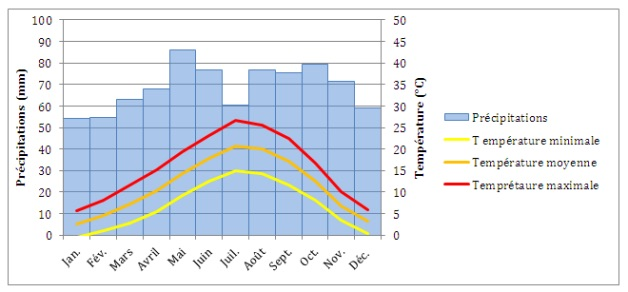
\includegraphics[width=0.6\textwidth]{graphics/DiagrammeThil.jpg}
\begin{tiny}

Graphique obtenu sur la page\\
\url{https://www.supagro.fr/ress-pepites/Opale/ECThil/co/1_SiteThil.html}\\
dernière visite le 31/10/2019.
\end{tiny}
\caption{Diagramme ombrothermique de Thil pour la période 2000-2013 (d'après InfloClimat)}
\label{fig:Expe}
\end{figure}


% Bibliographie
% Annexes éventuelles (en plus des 30 pages demandées)
\bibliographystyle{unsrt}
\bibliography{rapportPFE}
testtesttest


\appendix
\section{Données collectées.}


\section{Éléments majeurs de la conception.}

\section{Preuves de théorèmes.}
\end{document}
